\section{使用方法}
    软件端程序启动后应该出现如图\ref{client}所示界面,此时输入命令help可查看帮助。

    \begin{figure}[!hbp]
            \caption{软件端界面}\label{client}
            \centering
            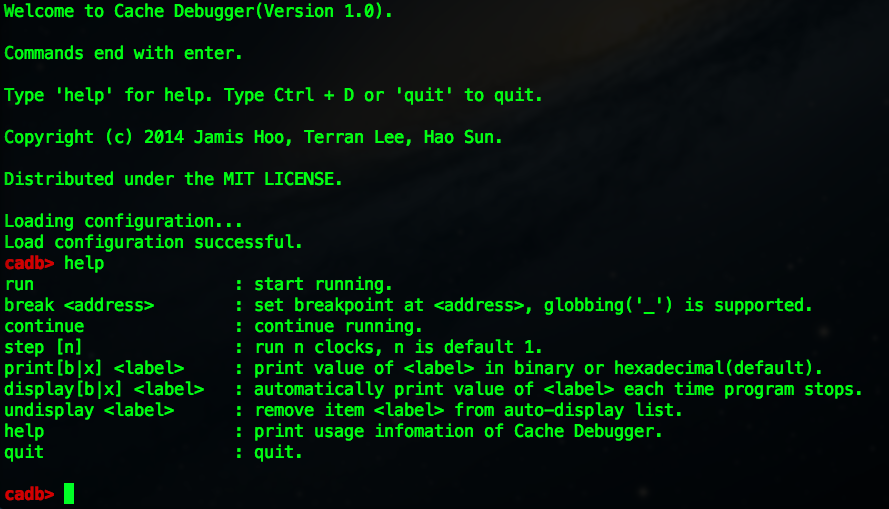
\includegraphics[width=\textwidth]{chart/cadb_client}
    \end{figure}

    所有支持的命令:
    \begin{enumerate}
    \item
    run: 开始运行。
    \item
    break <value>: 设置断点,支持十六进制(0x)和二进制(0b)。
    \item
    continue: 继续运行。
    \item
    step [n]: 前进n个时钟,n默认为1,支持二进制、八进制、十进制、十六进制。
    \item
    print[b|x] <label>: 以二进制(b)或十六进制打印变量。默认为十六进制。
    \item
    display[b|x] <label>: 自动打印变量。
    \item
    undisplay <label>: 取消所有该变量的自动打印。
    \item
    help: 显示帮助信息。
    \item
    quit: 退出。
    \end{enumerate}

    输入run相当于被调试模块得到一个reset信号后得到连续的时钟信号,%
    被调试模块应该在此条件下能正确运行。

    输入run、step、continue命令后程序会阻塞,%
    直到到达断点条件,用户才可继续操作,此时可使用print命令查看信号值。

    断点设置有高级用法,参见技术文档。

